%
The circle in Fig. \ref{fig:4.1.6_cir_1} is generated using the following python code 
\begin{lstlisting}
solutions/6/codes/circle/example/circle.py
\end{lstlisting}


The angle that the line makes with the $x$-axis is given by 
\begin{align}
\cos \theta = \frac{\myvec{1&-1}^T\myvec{1\\0}}{\norm{\myvec{1&-1}}\norm{\myvec{1&-1}}}
\\
&=\frac{1}{\sqrt{2}}
\\
\implies \theta = 45 \degree.
\end{align}
The area of the sector is then obtained as
\begin{align}
\frac{\theta}{360 \degree}\pi r^2 &= \frac{45 \degree}{360 \degree}\pi r^2 
\\
&= \frac{\pi}{8}
\end{align}
\begin{figure}[!ht]
\centering
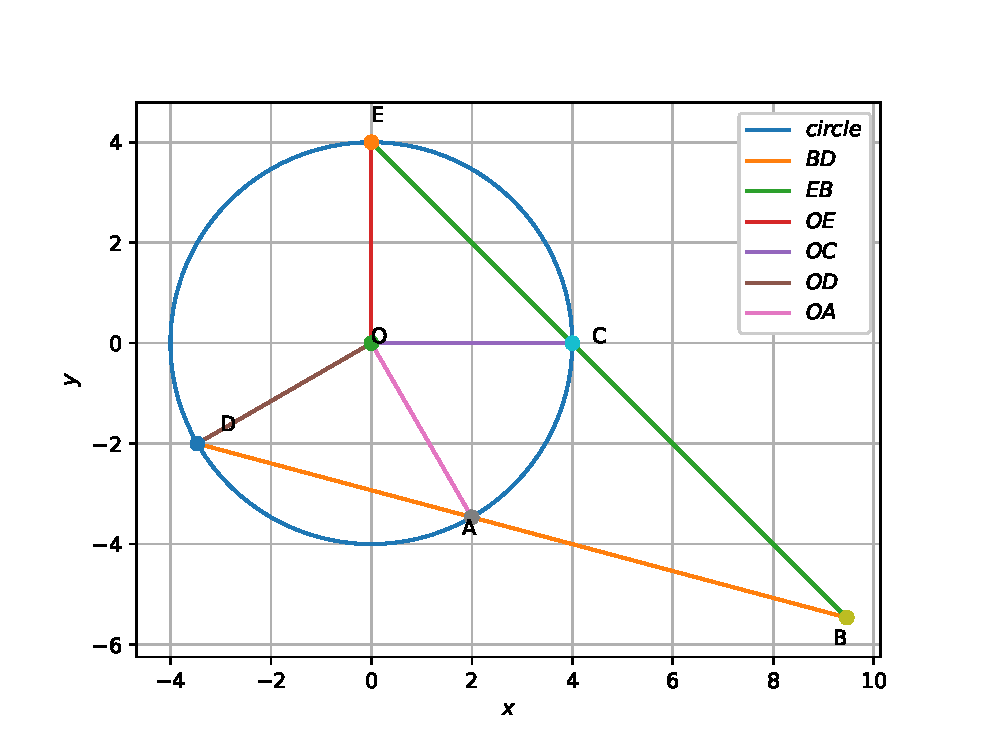
\includegraphics[width=\columnwidth]{./solutions/6/codes/circle/example/circle.eps}
\caption{Circle generated using python}
\label{fig:4.1.6_cir_1}
\end{figure}
